\section{Framework Implementation}
\label{sec:implementation}

In this section we describe the design of \sysname{}.
\sysname{} adds language support in \java{} virtual machines to
create and execute partitioned applications in enclaves.

\subsection{Partitioned \java{} Execution}

To executed partitioned applications,
\sysname{} creates two worlds of \java{} execution,
one in an enclave and one outside the enclave,
to execute code at different security levels.
Each world contains an individual \java{} vM.
We allow only classes that are part of a signed enclave images to
be executed inside the enclave,
and all the other classes of the application
must run outside the enclave and access the secured classes through
an interface exported by the enclave.

Using \java{} language to implement enclaves
has the benefit of minimizing the development or porting cost.
Consider partitioning a native application for enclaves.
There are two primary sources of development or porting cost:
Separating the security-sensitive code from all the remaining code,
and designing the interface between the two.
%\java{} classes have huge advantage on fulfilling both goals
%with minimal works, for two reasons:
\java{} classes are well modularized and are natural granularity for partitioning.
Public methods can be exported as
enclave interfaces, with proper type-checking of arguments.

%\sysname{} allows \java{} applications
%to easily model enclave support as part of the language,
%without the awareness of the native interface to architecture.
%To reflect this concept, we have implemented two key principles in the language support:
%\begin{compactenum}
\sysname{} models each enclave as an object,
both inside and outside the enclave.
The object is used to access enclave information and features,
such as retrieving security attestation.
Instantiating and interfacing with the isolated classes
in enclaves is transparent to the untrusted part of application,
except the first instantiation.

%For the untrusted side of an application, both the enclave itself and
%the classes isolated in the enclaves
%are encapsulated as black boxes, to which the application
%can request for isolated execution seamlessly.
%These objects can be passed as parameters to other methods,
%or even overrode to extend their functionalities.

\begin{figure}[t!]
\vspace{-0.1in}
\centering
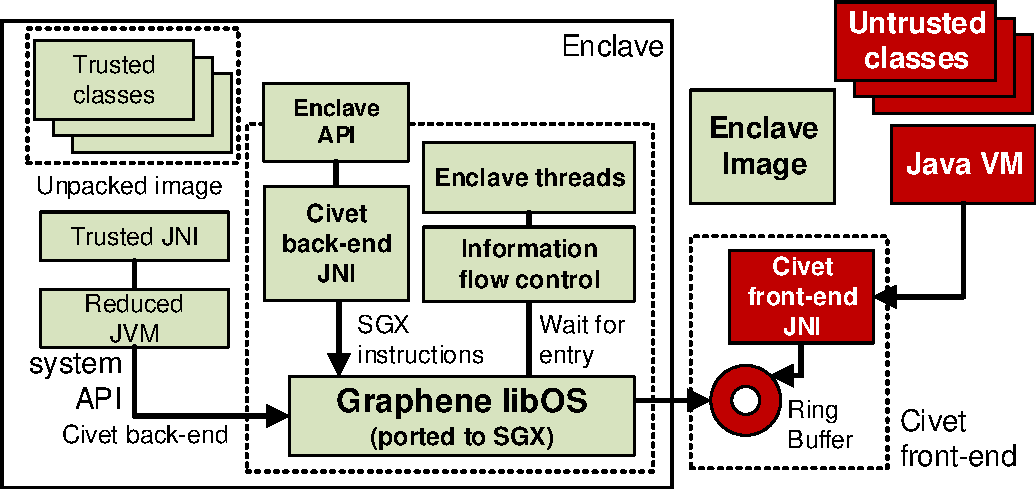
\includegraphics[width=3in]{civet-structure.pdf}
\vspace{-10pt}
\caption{\sysname{} framework overview. \sysname{} creates two worlds for an partitioned \java{} application, each with an individual JVM. The JVM in the enclave is ported using Graphene library OS. Untrusted classes can invoke methods of trusted classes through proxy objects, which will transparently access the enclave interface, through serialization and deserialization over an ring buffer accessed by both untrusted JVM and trust JVM. }
\label{fig:overview}
\end{figure}

\paragraph{Framework overview.} Figure ~\ref{fig:overview} shows the design and 
components of ~\sysname{} infrastructure.
All supporting classes to be isolated in the enclave
are packed into a JAR package --- an enclave image ---
and signed using a key given by the developers.
The untrusted side of the application initializes the enclave
using the enclave image JAR,
and starts to instantiate objects inside the enclave.
For each objects in the enclave, \sysname{} create a {\em proxy object} outside the enclave,
to access the interface exported from the enclave.
%and to represent the isolated objects to the rest of world.

The JVM running inside the enclave is a \jvmname{} VM
ported with the libOS-based programming model, using Graphene library OS.
Proxying isolated objects are handled through JNI in the untrusted JVM,
to access the low-level enclave interfaces.
To invocation of methods on the proxy objects are communicated
through a {\em ring buffer} outside the enclave memory,
accessible by both the enclave and the untrusted application.
The object ID, name of the invoking method, and all parameters are
serialized into binary forms and passed through the ring buffer.
In the enclave, one or more worker threads, initialized by the trusted JVM,
will poll the ring buffer,
accept the invocation requests,
de-serialize the parameters, invoke the method,
and return the result through the ring buffer.

%\begin{figure}[t!]
%\footnotesize
%\noindent
%\begin{minipage}[t]{.38\linewidth}
%\begin{lstlisting}[title=Isolated class,frame=none]
%class Secured {
%  Object run(
%    String args[]
%  ) {
%    ...
%  }
%}
%\end{lstlisting}
%\end{minipage}\hfill
%\begin{minipage}[t]{.54\linewidth}
%\begin{lstlisting}[title=Untrusted class,frame=none]
%class Untrusted {
%  static void main(
%    String[] args) {
%    Enclave e =
%      new Enclave(
%        "enclave.jar");
%    Secured o =
%      e.createInstance(
%        Secured.class);
%    Object r =
%      o.run(args);
%  }
%}
%\end{lstlisting}
%\end{minipage}
%\vspace{-10pt}
%\caption{Example code for using \sysname{} to interact with enclaves. Untrusted classes can use class {\tt Enclave} to create an enclave for a signed image JAR, and instantiate isolated object in the enclave. Invocation of methods of isolated objects will be proxied and forwarded into the enclave.}
%\label{fig:enclave-example}
%\end{figure}

Figure~\ref{fig:enclave-example} shows a code snippet that exercises such a framework.
The instance of class {\tt Enclave} represents the enclave created with
the given image JAR,
and is used to instantiated other isolated objects in the enclave.
Once isolated objects are instantiated,
\sysname{} also creates proxy objects outside the enclave.
All proxy objects belong to subclasses of the original classes,
so they can be casted to the superclasses
and passed around the untrusted application as arguments to other methods.

\paragraph{Limitations.}
Due to the limitations of \java{} class proxying,
untrusted classes cannot transparently invoke static methods
of isolated classes,
due to the ambiguity of which classes shall be accessed.
Also, enclave cannot execute any classes
that are not part of the enclave image JAR.
If untrusted classes passed a object
as the argument to an method of isolated classes,
and the class of the passed object is not part of the enclave image,
the framework will throw a ``Class Not Found'' exception.

\paragraph{Security Implications.}
The primary security implication of such a language support is to
improve {\em usability} of the security hardware.
By providing wrappers for security features and interfaces of an enclave,
developers can easily adopt enclaves into their programming models,
or override existing classes to leverage the hardware.
Because interaction with enclaves are mostly transparent
except the instantiation of first isolated objects,
developers need not to extensively modify existing code,
or constantly be aware of enclave interaction.
Yet all instantiated isolated objects will stay inside the enclave,
regardless of any further method invocation,
until the information flow filtering allows releasing the results.

Modeling the enclave support in language is also an improvement
for security policy specification.
Without language support, developers must constantly
keep partitioning in mind,
tracking whether the current location in code
will become part of the enclave,
because copying memory out of the enclave amy
violate the enclave's security policy.
In \sysname{}, developers use only minimal lines of code to
express the subjects that need to be put into the enclave,
and the framework will automatically isolate the subjects and any
of their products.  

%\sysname{} provides an encalve image utility that 
%takes a JAVA application JAR and a list of secure 
%classes as input, calculates transitive closure on 
%dependencies of those secure classes including system 
%classes, and outputs a JAR containing the trusted 
%secure JAVA classes and another JAR containing the 
%untrusted JAVA classes.
%The classes in the untrusted JAR are modified to use 
%proxy class replacements of the trusted classes.
%The utility also instruments the trusted JAVA classes 
%for information flow tracking.
%\sysname{} builds and cryptographically signs the 
%enclave to contain the Graphene LibOS, the trusted 
%JVM, JNI, information flow tracking library, and the 
%instrumented JAVA classes.

%At the runtime, the untrusted classes use 
%\sysname{} API to create and execute an enclave. 
%The \sgx{} hardware verifies the integrity of the 
%enclave code, and then starts the Graphene LibOS in 
%the enclave. Graphene loads the trusted JVM and JNI 
%in the enclave memory, and JVM runs the trusted JAVA 
%classes. The proxy objects and method calls are 
%passed between the enclave and untrusted world using 
%ring buffers. This communication channel is monitored 
%by the information filter to prevent any secure data 
%or other data derived from the secure data from 
%leaking to the untrusted world. The secret data and 
%code is provisioned in the enclave from the remote 
%servers after remote attestation using the 
%provisioning API of \sysname{}.

\subsection{Partitioning and Generating Images}

To initialize an enclave, the \sysname{} framework
loads an enclave image JAR containing all the supporting classes needed
for executing the isolated part of application.
The enclave image is a collection of all related classes in the developer's
environment as a snapshot, offered to the enclave
to recreate the stable, deterministic environment where the
developers have tested the application.
All loaded classes are part of the enclave's TCB,
so they must be signed by developers and verified by the infrastructure
during the runtime, to guarantee the integrity.

To minimize the effort for developers to package the supporting classes,
\sysname{} provides a building tool
to generate enclave image JARs,
%by collecting all required, supporting classes
from the developer's class paths.
The building tool
starts with one or more root classes given by the developer.
The root classes are the bottom line of enclave isolation,
and specify the boundary of partitioning.
The public methods of the root classes automatically
become part of the enclave interface.


Figure~\ref{fig:builder} shows the work flow of \sysname{}'s building tool.
The building tool takes an manifest file from the developers,
which specifies the class paths for the applications,
the root classes, and other attributes such as the signing key.
The tool recursively traces all dependency of the root classes,
until the supporting classes eventually converge.
Then, the supporting classes will be processed through
instrumentation and augmentation:
instrumentation adds information flow tracking in the classes,
and the augmentation adds an empty, dummy constructor to each class,
so their proxy objects create be instantiated.
After all previous steps, the tool packs all the collected classes,
signs them with the developer's key, and keep the public key
inside the image JAR. 

Automated partitioning in the \sysname{} building tool
covers most of the corner cases of dependency tracking.
There are exceptions such as
classes dynamically loaded using {\tt ClassLoader}s,
or subclasses that are not dependency of any class in the enclave.
%but developers intend to pass as a generalization of parameter types,
For these exceptions,
developers can specify additional classes to include in the enclave image.

\paragraph{Security Implications.}
By automating application partitioning,
\sysname{} can minimize the enclave TCB, more than
manual partitioning by developers.
Minimizing the TCB essentially reduce the attack factors in the enclave,
because any unused code can be effectively trimmed,
and any vulnerabilities in the trimmed code are eliminated.
As future work, \sysname{} can further reduce code by methods,
to even minimize the enclave TCB.

%\subsection{Providing Enclave Guarantees.}

\subsection{Enclave Infrastructure}

Beside initializing enclaves and partitioning \java{} applications,
\sysname{} also provides classes for access enclave infrastructure features.
Accessing enclave infrastructure features through classes
is both developer-friendly and platform-independent.

\paragraph{Wrappers to Architecture Features.}
\intel{} \sgx{} provides hardware-generated attestation
to prove the integrity of enclave,
and hardware-generated sealing keys
to encrypt data for permanent storage.
Accessing these features can be hard for \java{} classes,
because of the use of architecture-dependent instructions,
and cryptographical operations in both sides that request attestation.

\sysname{} provides methods like {\tt generateAttestation}
and {\tt verifyAttestation} in class {\tt Enclave}
to allow \java{} classes to conveniently access these features.
Attestation is especially needed for the enclave to open
a secured channel for communication with a remote, trusted service.
Once both sides of the communication have attested each other,
and guarantee the channel is securely encrypted,
the channel will be declassified from the information flow filtering,
and exempted from blocking for avoiding information leakage.

\paragraph{Secure Provisioning.}
Secure provisioning is a common step taken after remote attestation.
Most applications isolated in enclaves
needs to communicate with a remote, trusted service
to acquire certain security-sensitive resources.
The resources being provisioned are often encryption keys,
or sensitive information that needs to be processed.

\sysname{} provides classes called {\tt EnclaveProvServer}
and {\tt EnclaveProvClient}
to allow developers of enclaves to quickly build up
enclave provisioning services.
The server and client classes will transparently exchange attestation,
and create a secured channel.
Both the server and client can ship \java{} objects
to the other side,
while serialization, de-serialization and proper type-checking
will happen transparently.

\paragraph{Information Flow Filtering.}
Although the execution environment inside an enclave is isolated
from the system stacks and other applications,
it can still be vulnerable to information flow leakage,
if the execution is buggy.
\sysname{} effectively blocks information leakage
by applying information flow tracking and filtering, transparently
to the developers.

\sysname{} uses {\em Phosphor}~\cite{bell2014phosphor}
as the instrumentation framework for
tracking explicit and implicit information flow in isolated \java{} classes.
Explicit information flow is affected by direct assignment
and operations of objects.
Implicit information flow is affected by control flow that is determined by
branch conditions and method invocation.

By default, all classes in enclaves must be traced.
\sysname{} assumes
developers can easily make mistakes if
information flow tracking is an optional features.
To prevent human mistakes compromising the security of an enclave,
\sysname{} do not ask developers to annotate the classes
for tagging the objects,
but instead applies a whitelist-based policy:
\sysname{} will determine the tag of objects instatiated from a class,
based on a conservative default policy,
unless developers annotate the class as {\em not} security sensitive.

Once an object is tagged, the object contains secret that should not be
flown outside of the enclave.
\sysname{} blocks any possible information leakage on this object,
through two channels.
The first is the return values of enclave interface.
When the invocation to an enclave method from the untrusted application
is completed,
the trusted JVM will serialize the return value and
send it to the ring buffer.
The information flow filtering happens at the serialization:
if the to-be-serialized object is tainted by information flow,
either implicit or explicit,
the object will not be serialized and an ``Access Denied''
exception will be thrown.
The second channel of leaking information will be through
JNI calling system calls
to send data to files, pipes or sockets.
Because all system calls are intercepted by
Graphene library OS in the enclave,
the libOS can encrypted all outbound streams using a default enclave key.

\paragraph{Default Tagging Policy.}
Because \sysname{} only expect developers to make minimal modification
to the applications,
it will be excessive if it requires developers to
annotate every object that needs to be flown out of the enclave legally.
Fortunately, not all objects have to be tagged as secret since the beginning.
We design a conservative, default tagging policy,
which can skip tagging certain objects
if we are {\em absolutely} sure they contain no secret.
For instance, input arguments passed from the untrusted applications are
exempted from tagging.
Because the enclave image is visible outside the enclave,
methods and constants that come from the enclave image
will not contain any secret,
thus can be skipped for tagging.
Mostly, objects that are initially tagged are
objects that are generated in the enclave (e.g., a random number),
or objects that are provisioned from remote services.

\paragraph{Declassification.}
If the developers must send an object outside the enclave
regardless of the tag of the object,
the object has to be explicitly declassified.
A method {\tt release} in class {\tt Enclave} can declassify the tag
on an object.
Declassification is useful in many scenarios,
such as when developers use a provisioned key to encrypt a secret.
The information flow tracking will certainly tag the generated ciphertext
due to the information flow in the encryption algorithm.
However, because the encryption algorithm obfuscates the secret in the ciphertext,
the developers can explicitly declassify the object
to send it to network or permanent storage.

%Design Architecture

%\begin{figure}[t!]
%\centerline{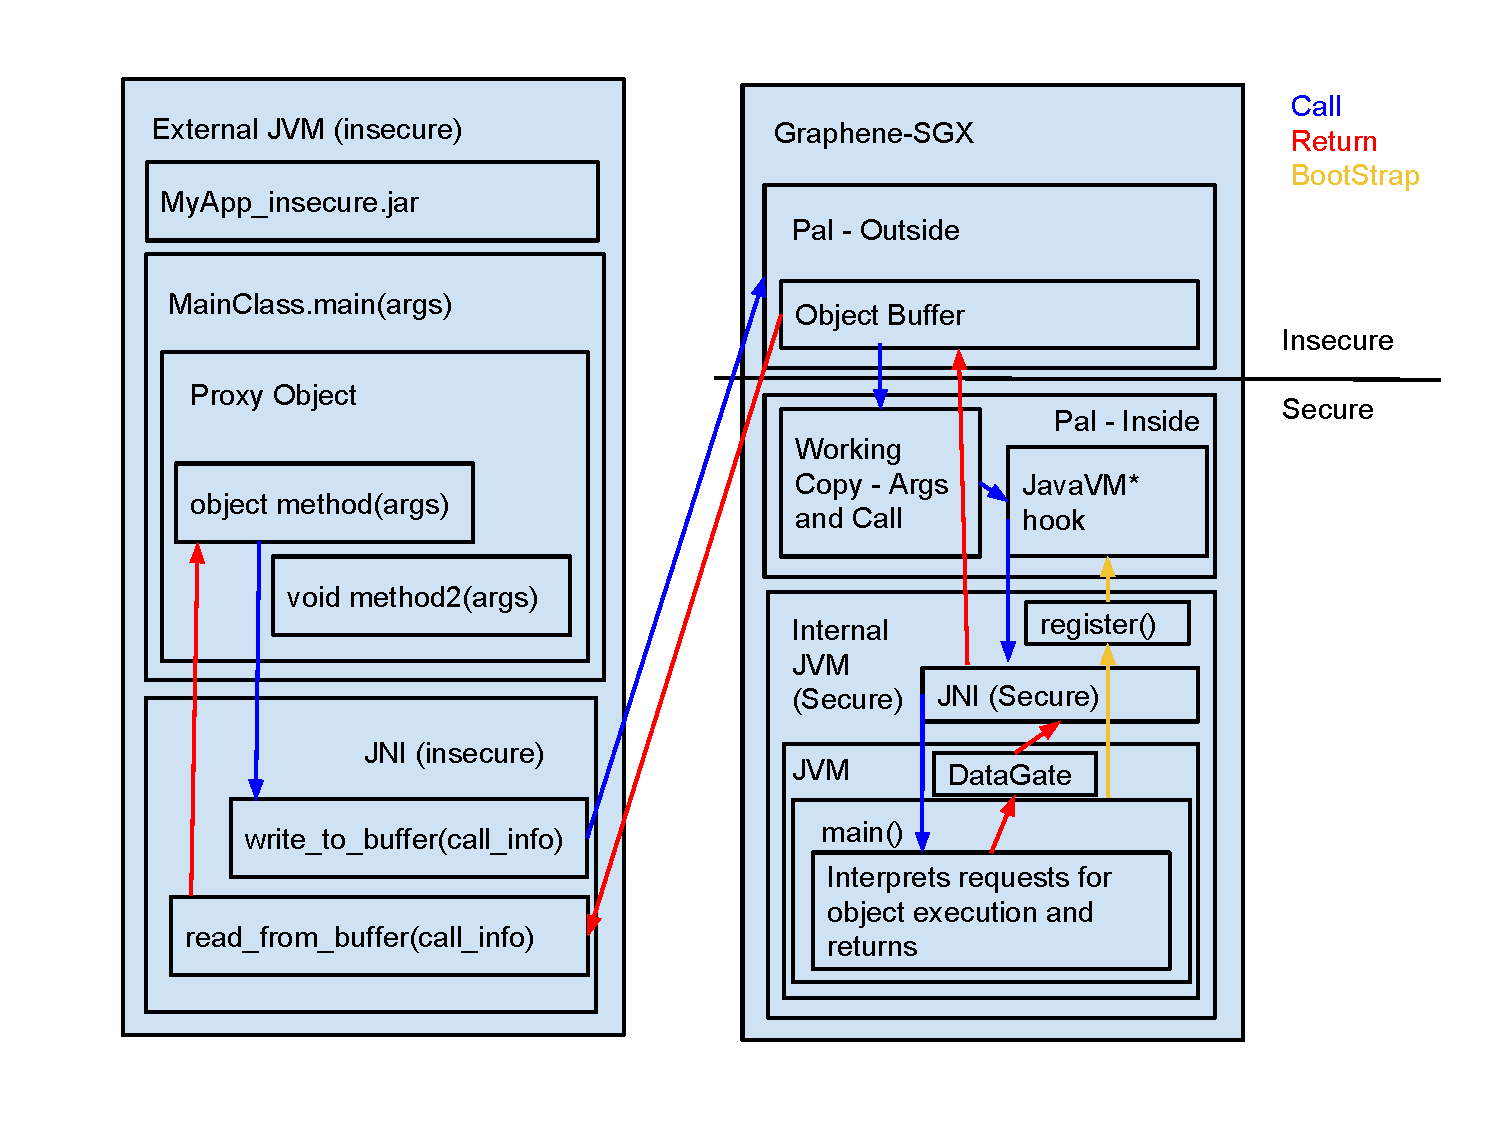
\includegraphics[width=\linewidth]{civet_flow.pdf}}
%\caption{Cevit Architecture and control flow.}
%\label{fig:architecture}
%\end{figure}

%\sysname{} leverages JAVA, a managed language 
%runtime, to help thwart the attacks discussed in 
%section~\ref{sec:background}. The modularity of JAVA 
%allows automatic partitioning of applications to 
%reduce the number of classes added to the Trusted 
%Computing Base. The type-safety property enforced by 
%JAVA runtime avoids exploitation of memory-safety 
%vulnerabilities in the application . JAVA framework 
%also eases the information flow tracking to prevent 
%information leakage due to buggy code. Moreover, 
%\sysname{} uses JAVA runtime to seamlessly 
%provision secure objects and classes in the enclave.




%\subsection{Automatic Partitioning of JAVA Applications}
%\subsection{Preventing Information Leakage}
%\subsection{Seamless Provisioning of Secure Objects and Classes}
